\documentclass{article}
\usepackage{xeCJK}
\setCJKmainfont{FandolSong} % Overleaf 自带的开源宋体
% Language setting
% Replace `english' with e.g. `spanish' to change the document language
\usepackage[english]{babel}

\usepackage{tabularx}
\usepackage{booktabs}

\usepackage{amsmath}  % 处理数学公式和 \text
\usepackage{amssymb}  % 处理 \mathbb 符号

% Set page size and margins
% Replace `letterpaper' with `a4paper' for UK/EU standard size
\usepackage[letterpaper,top=2cm,bottom=2cm,left=3cm,right=3cm,marginparwidth=1.75cm]{geometry}

% Useful packages
\usepackage{amsmath}
\usepackage{graphicx}
\usepackage[colorlinks=true, allcolors=blue]{hyperref}

\title{notes on VSRM}
\author{黎彩婷}

\begin{document}
\maketitle

\begin{abstract}
这是一篇关于《Promoting Efficient Reasoning with Verifiable Stepwise Reward》文章的解读笔记。
论文指出：大推理模型（LRM）虽推理能力强，但存在过度思考问题。通过 VSRM 这种分步奖励去监控它的思考过程。有效思考给奖，无效废话惩罚。
\end{abstract}

\section{引入}

先对本论文提到的LLM和LRM做一个区分：
\begin{table}[htbp]
    \centering
    \begin{tabular}{|p{2cm}|p{5cm}|p{5cm}|}
         维度&  LLM大语言模型& LRM大推理模型\\
         核心目标&  预测下一个Token，生成流畅、合理的文本& 通过多步推理解决复杂问题（数学、代码）\\
         工作模式&  直觉式生成：基于统计概率快速输出& 深思式推理：内部模拟思考链，可能伴随试错和回溯\\
         典型代表&  GPT-3.5& DeepSeek-R1\\
    \end{tabular}

  
\end{table}

基于人类反馈的强化学习模型（RLHF）训练分为三个阶段：预训练、奖励模型训练和强化学习微调。该论文提出的VSRM（Verifiable Stepwise Reward Mechanism）在奖励模型训练阶段被训练出来，在强化学习微调阶段作为奖励函数被调用，生成每一步的即时奖励。也就是说，它只是负责打分，优化算法（GIGPO/PPO）根据VSRM打出的分数，反向调整模型参数，让模型下次能得高分。

\begin{figure}[htbp]
\centering
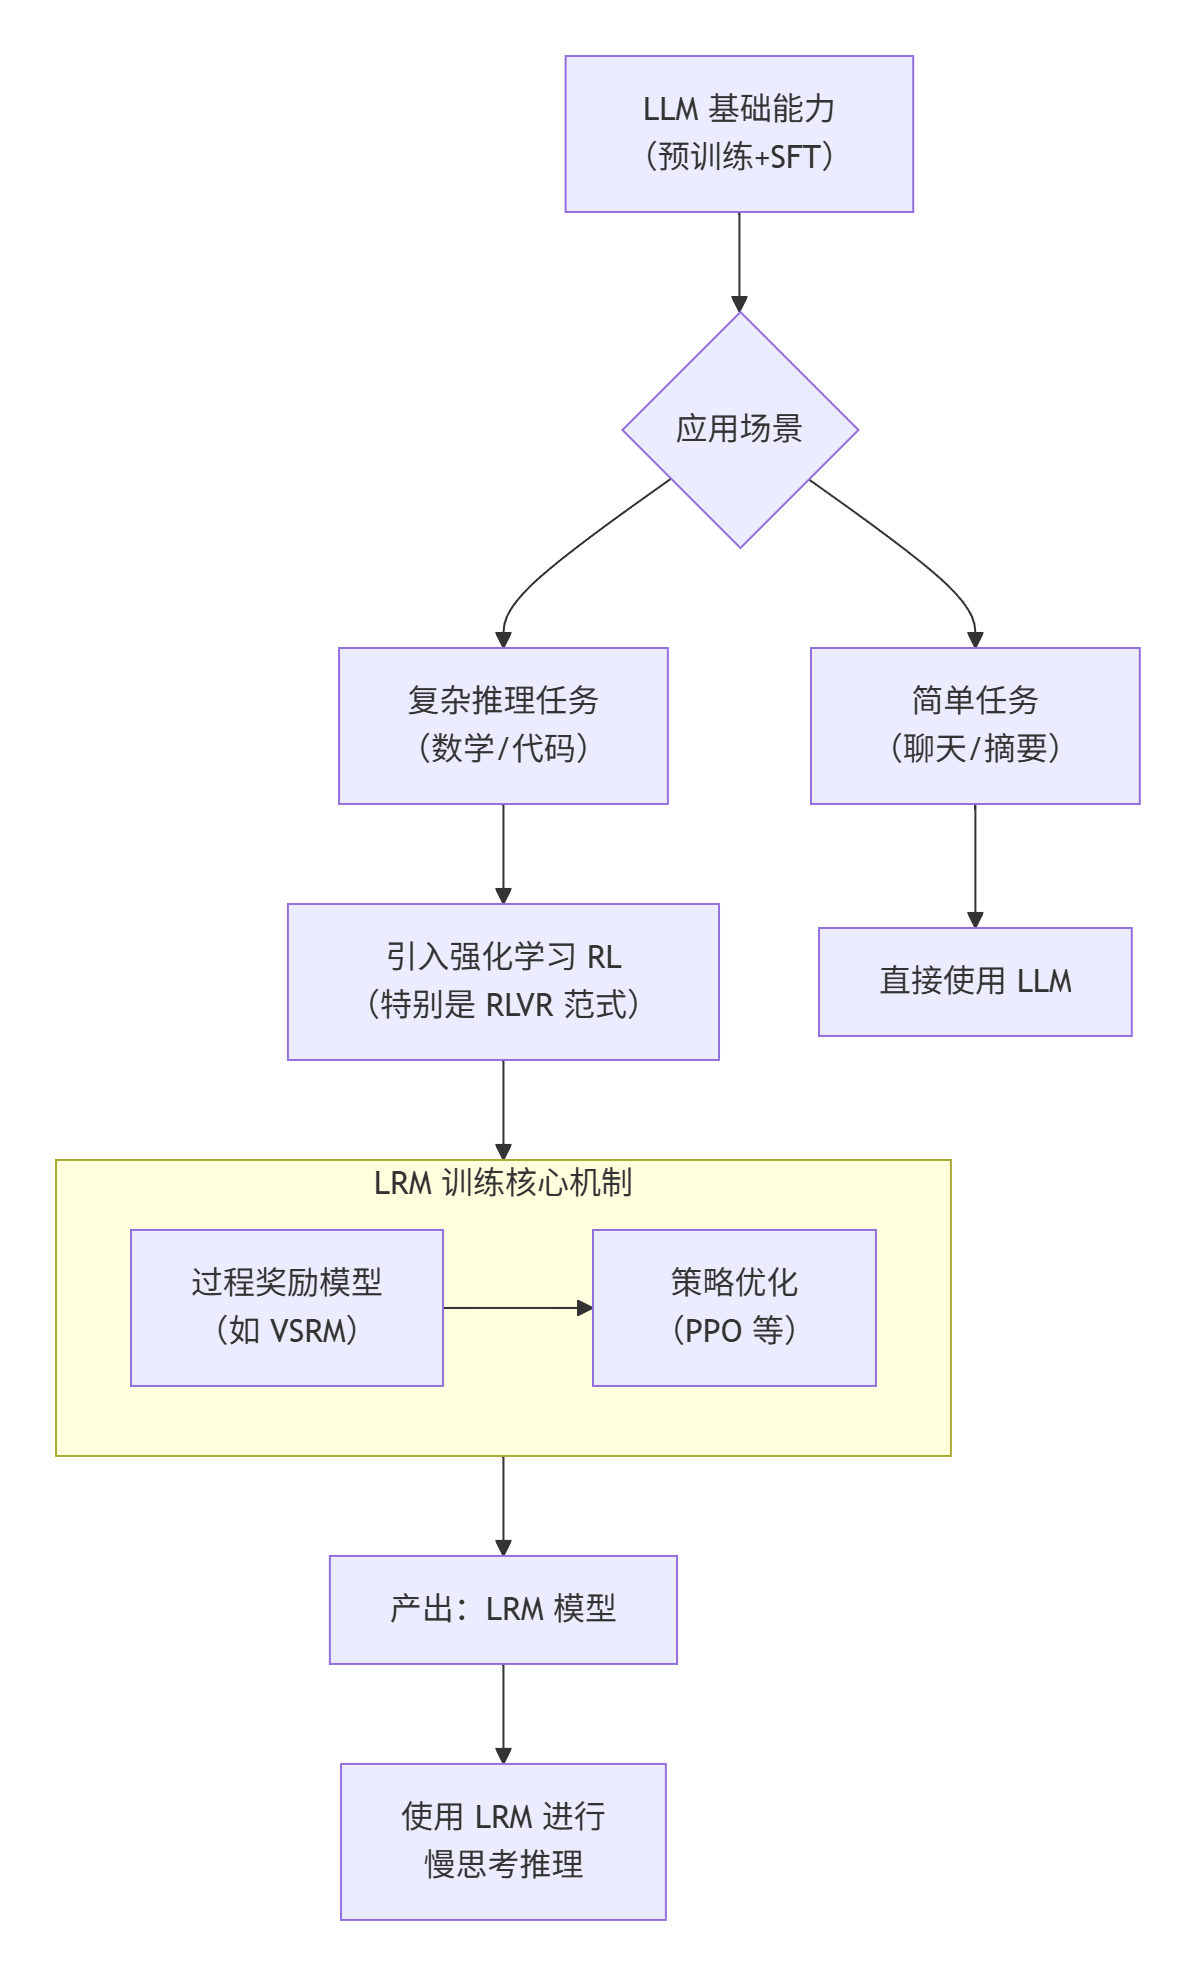
\includegraphics[width=0.5\linewidth]{p1.png}
\caption{\label{fig1}本图直观展示了从 LLM 到 LRM 的演变过程，以及VSRM在其中扮演的角色}
\end{figure}

\section{研究背景}

由引入部分的图表可知，LLM在复杂的推理任务中表现不佳，所以需要使用LRM。但由于LRM过度思考问题，导致token消耗量大，其未实现在实际应用中部署。
重新思考过度思考现象的本质：过度思考的一个关键表现是模型在中间步骤上花费大量计算，而这些步骤对最终准确性贡献甚微。鉴于复杂的推理任务本质上是一步步展开的，我们认为解决过度思考的根本方法是：鼓励中间步骤以提高准确性，同时惩罚无意义的步骤。 

\subsection{传统的奖励函数设计}
1.结果奖励 Result-based Reward
\begin{itemize}
    \item 根据最终结果的对错给出奖励。
    \item 对于中间步：rt=0 ; 对于最终步：rT=1（假设最终结果是正确的）。
\end{itemize}
2.过程奖励模型 Process Reward Model
\begin{itemize}
    \item 这是一个打分模型，给出每一步奖励 
    \item 依赖于该模型的准确率
\end{itemize}

以上无论是显式还是隐式，都将长度压缩纳入优化目标都可能削弱模型的推理能力。

\section{研究问题及方法}
VSRM，评估器。
我们重新思考过度思考现象的本质：计算复杂度与推理深度不匹配，找到了根本解决方案：鼓励有益的中间步骤，同时惩罚无效的步骤。 从而提升模型推理能力的同时，也不影响其性能。
\subsection{过度思考发生在什么时候？}
作者将推理过程划分为：问题重述、逐步解答、答案总结三个阶段，过度思考发生在逐步解答阶段。
作者将500道不同的题分别喂给两个模型生成回答，再由DeepSeek-R1 模型检测推理过程中的无效步骤。由下表可见：超一半的样本中显示出显著的无效步骤。因此，我们提出缓解过度思考的关键是准确区分有效和无效步骤，并将优化目标设定为鼓励有效步骤、惩罚无效步骤，从而实现高效的推理。 
\begin{figure}[htbp]
\centering
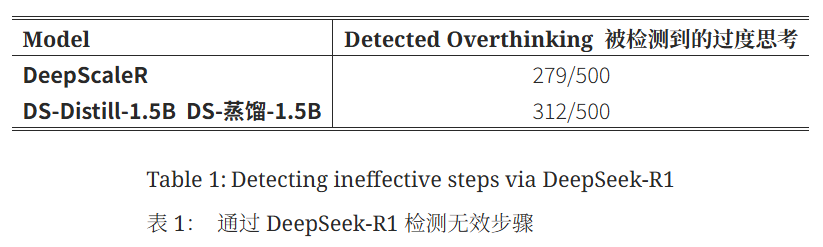
\includegraphics[width=0.75\linewidth]{p2.png}
\end{figure}

\subsection{VSRM分步处理流程}
\begin{enumerate}
    \item \textbf{自然推导}
    
    模型从头到尾写一遍，生成了一条完整的轨迹 $T$。

    \item \textbf{自动切分}
    
    VSRM根据模型推理过程中的“thus”、“so”、“wait”、“but”等特殊字样（记为集合 $S$），识别为一步推导的终点，并在此处将推理过程切分为多个子段。
    
    \begin{itemize}
        \item \textbf{注：} 相邻分割点间有最小间距；分割点必须位于包含特殊字段的\textbf{完整句子}的开头。
        \item \textbf{变量定义：}
        \begin{itemize}
            \item 分割点 $p=\{p_1,p_2,\dots,p_K\}$
            \item 完整轨迹为 ${T} = \{t_1, t_2, \dots, t_N\}$
            \item $T_{p_i}$：模型从开始到 $p_i$ 的所有记忆和逻辑进度的文本。
        \end{itemize}
        \item \textbf{中间状态：} 在时刻 $i$，模型所处的中间状态被严谨地定义为前缀子序列：
        \[ s_i = {T}_{p_i} = \{t_1, t_2, \dots, t_{p_i}\} \]
    \end{itemize}

    \item \textbf{子轨迹采样与推演}
    
    对于每一个中间状态 $s_i$：[问题] + $T_{p_i}$ + </think> 
    
    在每个分割点，模型会得到多个候选答案（从开始推理到当前步 $p_i$），计算这些候选答案的平均正确率 $\mathcal{A}_{\mathcal{T}_i}$。
    \begin{equation}
        \mathcal{A}_{\mathcal{T}_i} = \frac{1}{N} \sum_{j=i}^{N} \mathbb{I}(\text{IsCorrect}(\text{LRM}(\mathcal{T}_i)_j))
    \end{equation}
    其中，
    \begin{itemize}
        \item $LRM(T_i)_j$：LRM生成的第 $j$ 个候选答案；
        \item $IsCorrect(\dots)$：检验函数，将模型到第 $i$ 步推理出的第 $j$ 个答案和标准答案比对。如果一致返回True；否则返回False。
        \item $\mathbb{I}(\dots)$：指示函数。括号内是True返回1；否则返回0。
    \end{itemize}

    \item \textbf{价值审计与奖励分配}
    
    \textbf{治理过度思考的核心环节！}
    
    \begin{enumerate}
        \item[(1)] \textbf{价值审计}
        
        模型不看当前步的绝对胜率（正确率），而是看相比上一步的\textbf{胜率增量（价值增量）}：
        \[ d_i = \mathcal{A}_{\mathcal{T}_i} - \mathcal{A}_{\mathcal{T}_{i-1}} , i \in [1, \dots, k] \]
        \begin{itemize}
            \item 当 $i=1$ 时，$A_{T_1}$ 为只看题目的正确率；
            \item 当 $i=k$ 时，$d_k = A_T - A_{T_k}$，最后一步（$i=k$）"Therefore, the answer is..." 
            \item 如果 $d_k < 0$，则说明前面逻辑全对，但最后一步结论可能抄错了数字。
        \end{itemize}

        \item[(2)] \textbf{奖励分配}
        
        但是，在现实推理过程中，得出正确结论往往需要多个中间步骤的积累，而不是依赖单一的决定性行动。即 $A_i$ 在许多步骤中，可能保持不变，导致大多数位置 $d_i=0$，奖励信号稀疏。
        
        于是，VSRM引入了 $L_{max}$ (Lookahead Window)：
        
        如果第 $i-1$ 步的奖励 $|d_{i-1}|$ 极其微小（小于阈值 $\epsilon$），系统不会直接给 0。系统会往后看 $L_{max}$ 步。如果在第 $i+q-1$ 步，胜率突然\textbf{爆发式增长}了（超过了 $\epsilon$），说明前面那几步“铺垫”起到了关键的支撑作用。
        \[ r_{i-1} (\text{奖励}) = \underbrace{\text{sgn}(d_{i+q-1})}_{\text{是奖还是惩}} \cdot \underbrace{(|d_{i+q-1}| \cdot \gamma^q)}_{\text{打折后的力度}} \]
    \end{enumerate}

    \item \textbf{使输出符合可验证标准}
\end{enumerate}
由于一个token对应一个动作，所以需要\textbf{\textbf{将所有零散的奖励信号（逻辑分、结果分、格式分）打包成一个}与推理长度完全对等}的奖励序列：$R_{\mathcal{T}} = [\dots, r_1, \dots, r_t, \dots, r_k, \dots, r_{\mathcal{T}}^{\text{result}} + r_{\mathcal{T}}^{\text{format}}]$

\section{实验}
\subsection{实验装置}
\begin{itemize}
    \item 基座模型选择：经过知识蒸馏且具备初步思维链（CoT）能力的轻量化模型， \textbf{DS-Distill-1.5B/7B} 与 \textbf{DeepScaleR} 。
    \item 训练集：筛选覆盖各种难度且具备客观真值的合集：历史 AMC 问题（2023 年前）、Omni-MATH 数据集和 Still 数据集 。
    \item 评估集：1.覆盖范围广，MATH-500、AIME24、AIME25（问题解决艺术 \href{https://ar5iv.labs.arxiv.org/html/2508.10293?_immersive_translate_auto_translate=1\#bib.bib2}{2024}）、AMC23（美国数学协会 \href{https://ar5iv.labs.arxiv.org/html/2508.10293?_immersive_translate_auto_translate=1\#bib.bib20}{2023}）、Minerva（Lewkowycz 等 ，\href{https://ar5iv.labs.arxiv.org/html/2508.10293?_immersive_translate_auto_translate=1\#bib.bib15}{2022}） 和 OlympiadBench（Chaoqun 等 ，\href{https://ar5iv.labs.arxiv.org/html/2508.10293?_immersive_translate_auto_translate=1\#bib.bib3}{2024}）。 2.最大生成长度：20,000token. 3.温度和顶点：0.6，0.95，允许模型探索不同的解题路径。4.重复实验N：对于 MATH-500 和 OlympiadBench， N=16；对于其他基准测试 ，N=32.
    \item 计算框架部署：VeRL框架，应用了 PPO 和 Reinforce++算法 。
\end{itemize}
\subsection{主要结果分析}
pass@1：对于同一问题生成1个答案的平均准确率，衡量性能；Length：推理长度，衡量成本。
\begin{itemize}
    \item 基座模型：DS-Distill-1.5B
    观察 \textbf{DS-Distill-1.5B} 在 AIME24 上的表现：原始模型：pass@1 是 28.8，长度是 12605。\textbf{VSRM-R++}：pass@1 提升到 \textbf{29.5}，但长度直接砍掉了一半，只有 \textbf{6958}（减少了 5647 个 token） 。其实现了性能提升与成本压缩的双重收益。  
\end{itemize}
\begin{figure}[htbp]
\centering
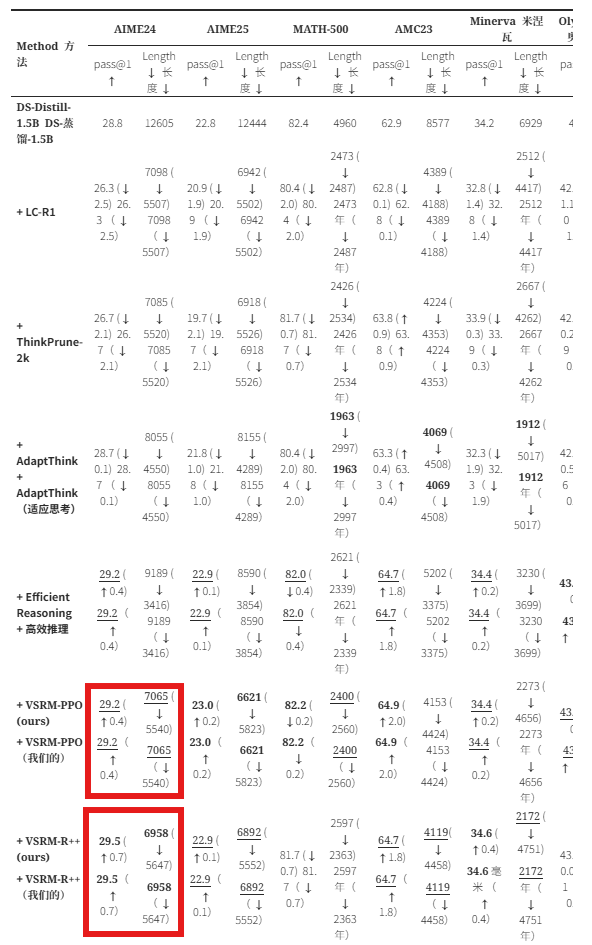
\includegraphics[width=0.75\linewidth]{2026-04-02 114853.png}
\end{figure}
\begin{itemize}
    \item 基座模型：DS-Distill-7B
    \textbf{VSRM-PPO：} 表现非常稳健，在 7B 模型上，长度压缩极其激进（例如在 AIME25 上砍掉了近 4000 个 token，准确率还反升了 0.2）。 虽然在AIME24中，准确率不如除了LC-R1的其他模型，但仍然节约了大量token。这种下降本质上是\textbf{用 1.3\% 的准确率损失，换取了约 35\% 的算力成本节省}。在工业界看来，这往往是一个非常成功的优化。
\end{itemize}
\begin{figure}[htbp]
\centering
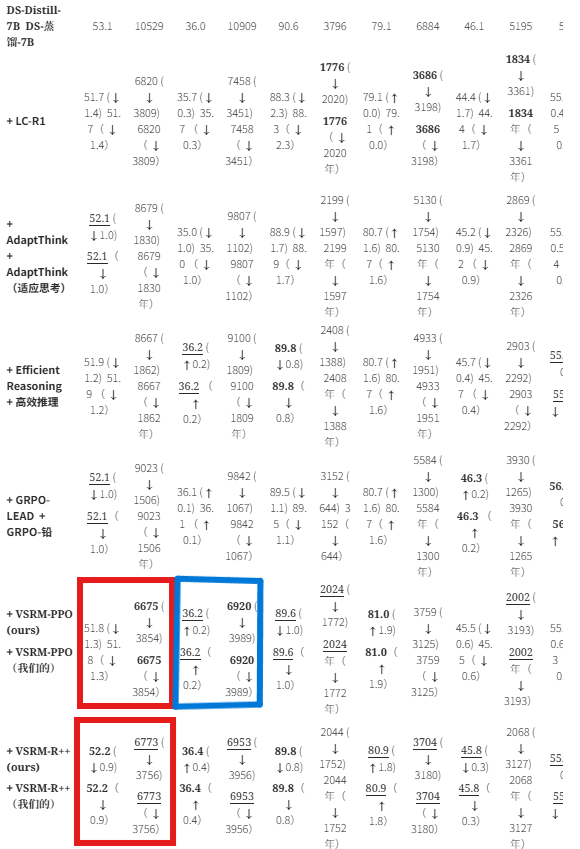
\includegraphics[width=0.75\linewidth]{2026-04-02 115025.png}
\end{figure}
\begin{itemize}
    \item 基座模型：DeepScaleR
    结果显示，VSRM 在所有基准测试中压缩输出长度，同时保持接近原始 DeepScaleR 的性能。相比之下，尽管 ThinkPrune-2k 实现了更大幅度的输出长度缩减，但它削弱了 DeepScaleR 强大的推理能力，这与解决过度思考问题的初衷背道而驰。
\end{itemize}
\begin{figure}[htbp]
\centering
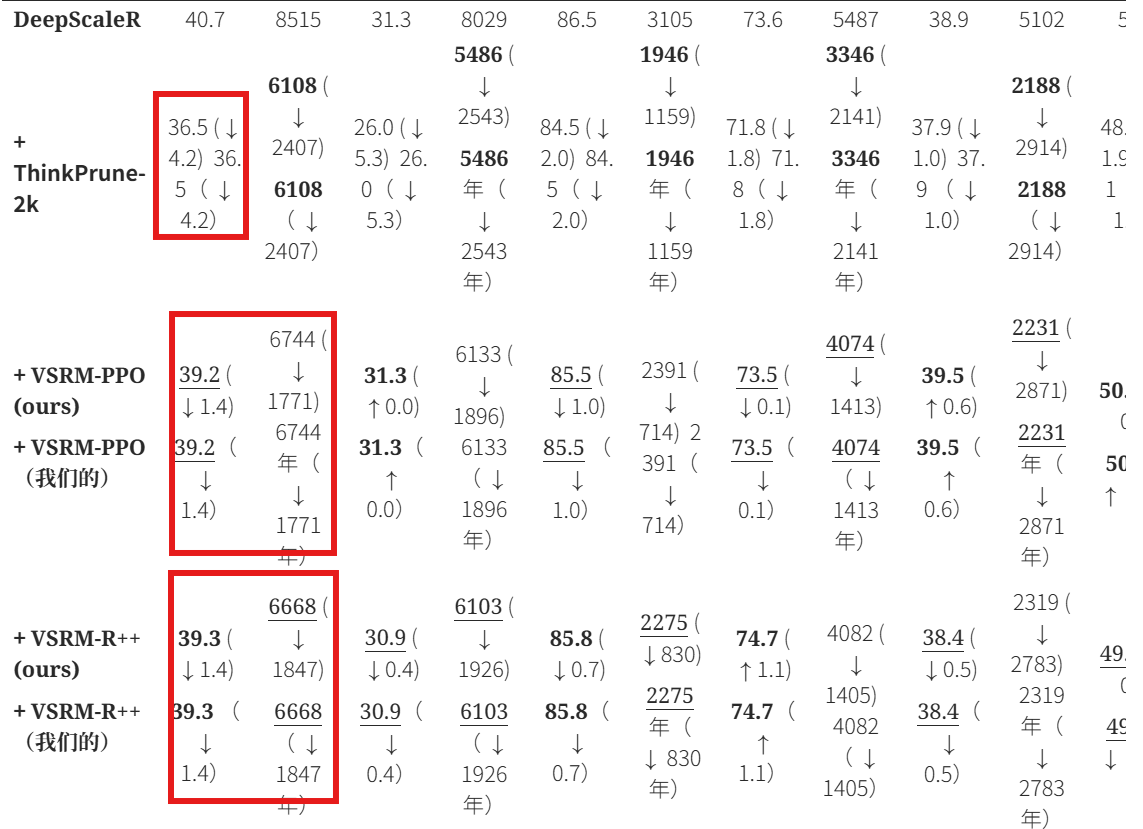
\includegraphics[width=0.75\linewidth]{2026-04-02 115656.png}
\end{figure}
在所有实验结果中，论文的方法始终如一地减少了冗余输出，缓解了各种规模和类型模型的过度思考问题，同时保持了原始的推理能力。在所有比较方法中，VSRM 在性能与效率之间取得了极佳的平衡，证明了其在根本上解决过度思考问题方面的优势。 
\subsection{消融实验} 
在上一小节通过VSRM和其它方法对比，可知其能有效解决过度思考问题。那么这一小节分析具体是VSRM中的哪个机制起到关键作用。
w/o decay和VSRM-PPO（完整版的对比），可见传播衰减机制的重要性：\[ r_{i-1} (\text{奖励}) = \underbrace{\text{sgn}(d_{i+q-1})}_{\text{是奖还是惩}} \cdot \underbrace{(|d_{i+q-1}| \cdot \gamma^q)}_{\text{打折后的力度}} \]

\begin{table}[htbp]
    \centering
    \small % 略微调小字体，让文字换行更自然
    \caption{不同实验版本的性能与长度对比 (AIME25)}
    \label{tab:vsrm_results}
    
    \begin{tabularx}{\textwidth}{lXX} % 三线表通常不需要竖线 |
        \toprule % 顶部粗线
        \textbf{实验版本} & \textbf{核心逻辑} & \textbf{实验表现 (AIME25)} \\
        \midrule % 中间细线
        Baseline & 原始蒸馏模型，无强化学习。 & $Pass@1: 22.8$ \quad $Length: 12444$ \\
        \addlinespace % 增加行间距，防止文字太挤
        Original PPO & 仅采用二元结果奖励（对/错）。 & 性能微升，长度略减（格式约束所致）。 \\
        \addlinespace
        w/ penalty & 采用显式\textbf{长度惩罚}函数。 & \textbf{性能暴跌} ($20.9$)，长度压缩效果不如 VSRM。 \\
        \addlinespace
        w/o decay & 有步骤奖励，但\textbf{无传播衰减}机制。 & 长度抑制能力受限，无法有效区分无效步骤。 \\
        \addlinespace
        \textbf{VSRM-PPO} & \textbf{完整版}：含步级奖励 + 传播衰减。 & \textbf{性能最高} ($23.0$)，\textbf{长度最精简} ($6621$)。 \\
        \bottomrule % 底部粗线
    \end{tabularx}
\end{table}

\subsection{推理行为分析}
在上面两节实验中，我们足以见识到VSRM对推理准确性和性能上的提升，那么回归问题的原始：它是否解决了过度思考问题呢？下表结果可以回答这个问题。
\begin{figure}[htbp]
\centering
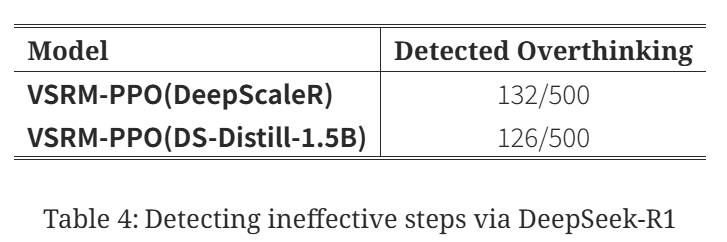
\includegraphics[width=0.75\linewidth]{2026-04-03 194040.png}
\end{figure}
那么，overthinking问题得到了有效缓解，那么是否会导致underthinking呢？
由下图可见，随着k的增加，对于N个不同问题的k个回答的准确率也在逐渐上升。可见推理并没有僵化，模型在探索不同问题解决方法方面的多样性。
\begin{figure}[htbp]
\centering
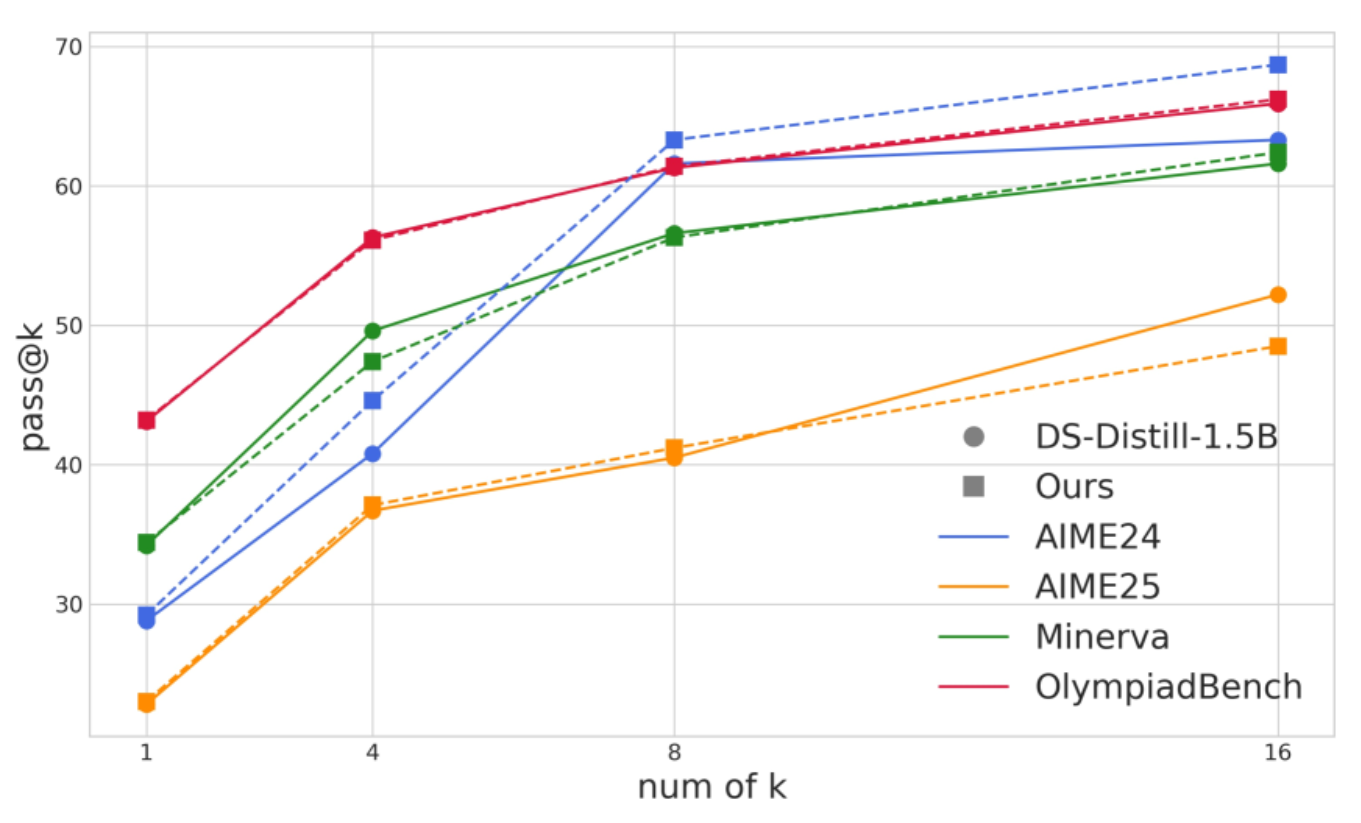
\includegraphics[width=0.75\linewidth]{2026-04-03 194519.png}
\end{figure}

\section{结论}
本论文聚焦于LRM的过度思考问题，并重新审视其本质：提议将“鼓励有效的中间步骤并惩罚无效步骤”作为优化目标。基于这一见解，作者引入了一种可验证的逐步奖励机制，根据推理轨迹中中间状态的表现，将逐步奖励分配给特定位置。并在多个基准测试中对数学问题进行的大量实验验证了此见解。该方法不仅显著缓解了过度思考的问题，还保留了——甚至在某些情况下略微增强——模型的原始推理能力，实现了高效的推理。 

\section{局限性}
在工程实践中，由于本实验所采用的 VSRM 奖励机制高度依赖于数据结果的客观真值，这确实引出了一个核心矛盾：当模型为实现目标输出而过度简化逻辑路径（即 Underthinking）时，用户往往因缺乏基准方案而难以察觉其在资源成本或架构扩展性上的次优性。尽管 Pass@k 实验证明了模型在压缩输出长度的同时仍保留了探索多种解题路径的智力多样性，但在缺乏显式“成本奖励函数”如：$$Reward_{final} = Reward_{correct} - \lambda \cdot \text{Time\_Complexity}$$的情况下，模型倾向于达成“结果正确”这一最低限度的胜率反馈，而非追求全局最优的经济性方案，这便构成了推理模型从逻辑正确向工程卓越演进中的关键局限。
比如，在用AI做项目涉及到算法时，虽然能得到理想的输出，但是得到的不一定时最省钱的方案。
\textbf{Underthinking 的隐患：} 模型可能为了追求这个“正确结果”，选择了逻辑最简单、最粗暴的实现方式。例如：
\begin{itemize}
    \item 它用 $O(n^2)$ 的算法解决了本应用 $O(n log n)$ 解决的问题。
    \item 它调用了昂贵的 API 组合，而不是寻找更廉价的平替。
\end{itemize}
但是引入成本奖励函数的话，在模型训练上的成本可能会增大，虽然在推理时能节约一定成本，这需要定量分析。
\end{document}
